\begin{figure}[H]
	\centering
	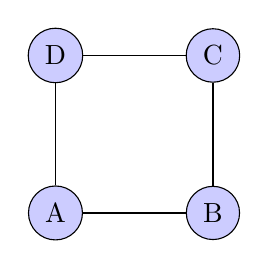
\begin{tikzpicture}
		\node[circle, draw, fill=blue!20] (A) at (0,0) {A};
		\node[circle, draw, fill=blue!20] (B) at (2,0) {B};
		\node[circle, draw, fill=blue!20] (C) at (2,2) {C};
		\node[circle, draw, fill=blue!20] (D) at (0,2) {D};
		
		\draw (A) -- (B);
		\draw (B) -- (C);
		\draw (C) -- (D);
		\draw (D) -- (A);
	\end{tikzpicture}
	\caption{Cyclic graph example with a cycle A-B-C-D-A.}
	\label{fig:cyclic-graph}
\end{figure}
